\begin{solution}{Question 1}\label{ques:1}
    \begin{question}
    Given an alphabet $\Gamma = \{l_1,...,l_k\} $, construct an NFA that accepts strings that don’t have all the characters from $\Gamma$. Can you give an NFA with $k$ states?
    \end{question}
    \tcblower{}
    \begin{proof}[Solution]
    We have to construct an $NFA$ such that the string $(x)$ to be accepted has atmost $k-1$ unique letters used out of language $\Gamma$. The regular expression for the problem can be defined as $x = [l_1-l_{k-1}]^*+ [l_1-l_{k-2}l_k]^* + [l_1-l_{k-3}l_{k-1}-l_{k}]^* + \dots + [l_2-l_k]^*$\\
    (where + is a union and we are following code regex syntax)\\
    For every regular expression, we can define an $\epsilon-NFA$. The $NFA (Q, \Gamma, \delta, q_0, F)$ created by aforementioned regular expression is defined by following diagram:
    \begin{center}
        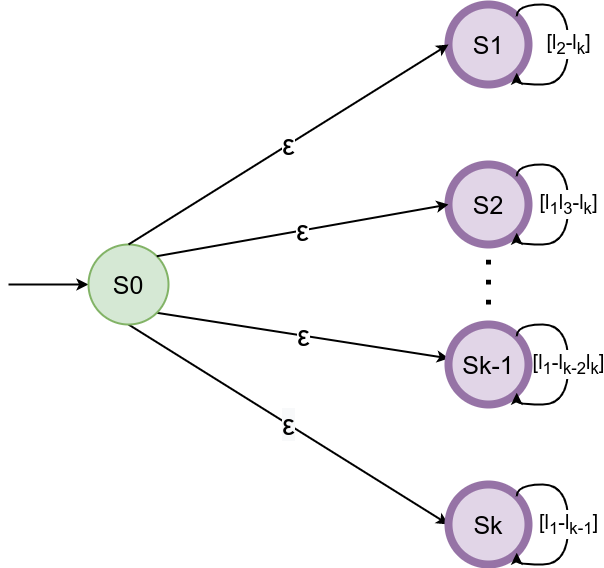
\includegraphics[scale=0.6]{NFA.png}
    \end{center}
    
    
    \end{proof}
\end{solution}
